\documentclass[10pt]{article} 

\parskip 6pt
\parindent 0pt

\usepackage[yyyymmdd,hhmmss]{datetime}
\usepackage{fullpage}
\usepackage{mdframed}
\usepackage{enumitem}
\usepackage{lineno}
\usepackage[explicit]{titlesec}
%\usepackage{url}
\usepackage{hyperref}
\usepackage{graphicx}
\usepackage{graphviz}
\usepackage[colorinlistoftodos,prependcaption,textsize=normal]{todonotes}
\newcommand{\TODO}[2][]{\todo[color=red!10,inline,#1]{#2}}
\newcommand{\GE}{\TODO{Grammar}}
\newcommand{\SE}{\TODO{Spelling}}
\newcommand{\TE}{\TODO{Term}}
\newcommand{\CE}{\TODO{Citation}}
\usepackage{listings}
\usepackage{minted}
\usepackage[most]{tcolorbox}
\usepackage{lastpage}
\usepackage{multicol}
\usepackage{enumitem}
\usepackage{makecell}
%\usepackage{cmap}
 \usepackage{microtype}
    \DisableLigatures[f]{encoding=T1}
\usepackage[T1]{fontenc}

\titleformat{\section}
  {\large\sffamily\bfseries}
  {\thesection.}
  {0.5em}
  {\MakeUppercase{#1}}
  []
\titleformat{name=\section,numberless}
  {\large\sffamily\bfseries}
  {}
  {0em}
  {\MakeUppercase{#1}}
  []
\titleformat{\subsection}
  {\sffamily\bfseries}
  {\thesubsection.}
  {0.5em}
  {#1}
  []
\titleformat{\subsubsection}
  {\sffamily\small\bfseries\itshape}
  {\thesubsubsection.}
  {0.5em}
  {#1}
  []
\titleformat{\paragraph}
  {\sffamily\small\bfseries}
  {\theparagraph}
  {1em}
  {#1}
  []
\titleformat{\subparagraph}
  {\sffamily\small\bfseries}
  {\thesubparagraph}
  {1em}
  {#1}
  []
\titlespacing*{\section}{0pc}{3ex \@plus4pt \@minus3pt}{5pt}
\titlespacing*{\subsection}{0pc}{2.5ex \@plus3pt \@minus2pt}{2pt}
\titlespacing*{\subsubsection}{0pc}{2ex \@plus2.5pt \@minus1.5pt}{2pt}
\titlespacing*{\paragraph}{0pc}{2ex \@plus2.5pt \@minus1.5pt}{2pt}
\titlespacing*{\subparagraph}{0pc}{2ex \@plus2.5pt \@minus1.5pt}{2pt}



\newcommand{\tightlist}{}

\tcbuselibrary{minted}

% \definecolor{codebggray}{rgb}{0.95,0.95,0.95}
\definecolor{codebggray}{rgb}{1.0,1.0,1.0}


\newcounter{filePrg}


\tcbuselibrary{listings}
\tcbuselibrary{minted}

\newtcbinputlisting[use counter=filePrg, number within=section, list inside=lol]{\codeFromFile}[4]{%
  listing engine=minted,
  minted language=#1,
  listing file={#2},
  minted options={autogobble,linenos,breaklines},
  listing only,
  size=title,
    drop fuzzy shadow,
  breakable,
  enhanced jigsaw,
    %arc=1.5mm,
  %colframe=brown,
  %coltitle=White,
  %boxrule=0.5mm,
  %colback=white,
  %coltext=Black,
  title={Listing \thetcbcounter : #3 \hfill%
    \smash{\raisebox{-6pt}{\includegraphics[width=.5cm,height=.5cm]{images/code2.png}}}},
    list entry=Listing~\thetcbcounter : #3,
    %OR next two lines
    %title={Listing \thetcbcounter : #3},
    %overlay={\node[anchor=north east,outer sep=-9pt] at ([xshift=-25pt]frame.north east) {\includegraphics[width=1cm,height=1cm]{images/code2.png}}; },
  label=lst:#4
}

\newtcbinputlisting[use counter=filePrg, number within=section, list inside=lol]{\codeFromJson}[4]{%
  listing engine=minted,
  minted language=#1,
  listing file={../cloudmesh/specification/examples/#2},
  minted options={autogobble,linenos,breaklines},
  listing only,
  size=title,
  %  drop fuzzy shadow,
  breakable,
  enhanced jigsaw,
    %arc=1.5mm,
  colframe=black!10,
  coltitle=black,
  %boxrule=0.5mm,
  % colback=black!5,
  colback=white,
  coltext=black,
  title={Object \thetcbcounter : #3 \hfill%
    \href{https://github.com/cloudmesh/cloudmesh.rest/blob/master/cloudmesh/specification/examples/#2}{\smash{\raisebox{-6pt}{\includegraphics[width=.5cm,height=.5cm]{images/code2.png}}}}},
    list entry=Object~\thetcbcounter : #3,
    %OR next two lines
    %title={Listing \thetcbcounter : #3},
    %overlay={\node[anchor=north east,outer sep=-9pt] at ([xshift=-25pt]frame.north east) {\includegraphics[width=1cm,height=1cm]{images/code2.png}}; },
  label=#4
}

\renewcommand{\contentsname}{Table of Contents}
%\renewcommand{\lstlistingname}{List of Objects}
%\renewcommand{\lstlistlistingname}{List of Objects}
\renewcommand\listoflistingscaption{List of Objects}

\makeatother

\setcounter{secnumdepth}{6}
\setcounter{tocdepth}{6}



\title{NIST Big Data Interoperability Framework: Volume 8, Interfaces}

\author{Gregor von Laszewski,Fugang Wang, Badi Abdhul-Wahid, 
        Wo L. Chang}

\date{Draft v0.0.1, \today} 


\begin{document}

%%%%%%%%%%%%%%%%%%%%%%%%%%%%%%%%%%%%%%%%%%%%%%%%%%%%%%%%%%%%%%%%%%%%%%
% FRONTPAGES 
%
%\newpage
%\listoftodos[Notes]
%\newpage

%%%%%%%%%%%%%%%%%%%%%%%%%%%%%%%%%%%%%%%%%%%%%%%%%%%%%%%%%%%%%
% PAGE 1
%%%%%%%%%%%%%%%%%%%%%%%%%%%%%%%%%%%%%%%%%%%%%%%%%%%%%%%%%%%%%
\begin{flushright}
{\Large\bf NIST Special Publication 1500-8} 

\bigskip\bigskip

\hrule
\bigskip\bigskip

{\Huge\bf {\sf
NIST Big Data Interoperability Framework:

\bigskip

Volume 8, Reference Architecture Interface
}}


\bigskip\bigskip
\hrule

\vspace{2cm}

{\large

NIST Big Data Public Working Group

Standards Roadmap Subgroup

\vspace{2cm}

Draft Version 1, Revision 1 

\today, \currenttime

\url{https://bigdatawg.nist.gov/V2_output_docs.php}
 
\bigskip


\bigskip

\bigskip

\bigskip
\url{http://dx.doi.org/10.6028/NIST.SP.1500-8}

}
\vspace{2cm}

\vfill

\begin{flushright}
\includegraphics{images/nist.png}
\end{flushright}

\end{flushright}

\newpage



%%%%%%%%%%%%%%%%%%%%%%%%%%%%%%%%%%%%%%%%%%%%%%%%%%%%%%%%%%%%%
% PAGE 2
%%%%%%%%%%%%%%%%%%%%%%%%%%%%%%%%%%%%%%%%%%%%%%%%%%%%%%%%%%%%%

\begin{flushright}
NIST Special Publication 1500-6

Information Technology Laboratory

\bigskip 

{\Huge\bf\sf NIST Big Data Interoperability Framework:

\bigskip

Volume 8, Reference Architecture Interface
}

\bigskip

{\bf Version 0.1}

\bigskip \bigskip \bigskip \bigskip \bigskip \bigskip

NIST Big Data Public Working Group (NBD-PWG)

Reference Architecture Subgroup

National Institute of Standards and Technology

Gaithersburg, MD 20899

\bigskip

\url{http://dx.doi.org/10.6028/NIST.SP.1500-8}

\bigskip

\today

\vfill

\begin{flushright}
\includegraphics{images/dep-commerce.png}
\end{flushright}

 
U. S. Department of Commerce

{\it Penny Pritzker, Secretary}

\bigskip
National Institute of Standards and Technology

{\it Willie May, Under Secretary of Commerce for Standards and Technology and Director}
\end{flushright}
\newpage



%%%%%%%%%%%%%%%%%%%%%%%%%%%%%%%%%%%%%%%%%%%%%%%%%%%%%%%%%%%%%%%%%%%%%%
% PAGE 3
%%%%%%%%%%%%%%%%%%%%%%%%%%%%%%%%%%%%%%%%%%%%%%%%%%%%%%%%%%%%%%%%%%%%%%

\
\begin{center}
{\bf National Institute of Standards and Technology (NIST) Special
  Publication 1500-8}

\pageref{LastPage} pages (\today)
\end{center}

\begin{mdframed}[backgroundcolor=black!5,topline=false,bottomline=false,rightline=false,leftline=false]

  Certain commercial entities, equipment, or materials may be
  identified in this document in order to describe an experimental
  procedure or concept adequately. Such identification is not intended
  to imply recommendation or endorsement by NIST, nor is it intended
  to imply that the entities, materials, or equipment are necessarily
  the best available for the purpose.

  There may be references in this publication to other publications
  currently under development by NIST in accordance with its assigned
  statutory responsibilities. The information in this publication,
  including concepts and methodologies, may be used by federal
  agencies even before the completion of such companion
  publications. Thus, until each publication is completed, current
  requirements, guidelines, and procedures, where they exist, remain
  operative. For planning and transition purposes, federal agencies
  may wish to closely follow the development of these new publications
  by NIST.

  Organizations are encouraged to review all draft publications during
  public comment periods and provide feedback
  to NIST. All NIST publications are available at \\
  \url{http://www.nist.gov/publication-portal.cfm}.

\end{mdframed}

\bigskip \bigskip \bigskip

\begin{center}
{\bf Comments on this publication may be submitted to Wo Chang}
\bigskip

National Institute of Standards and Technology

Attn: Wo Chang, Information Technology Laboratory

100 Bureau Drive (Mail Stop 8900) Gaithersburg, MD 20899-8930

Email: SP1500comments@nist.gov 
\end{center}

\newpage


%
%
%%%%%%%%%%%%%%%%%%%%%%%%%%%%%%%%%%%%%%%%%%%%%%%%%%%%%%%%%%%%%%%%%%%%%%

\section*{\hfill Request for Contribution \hfill}

The NIST Big Data Public Working Group (NBD-PWG) requests
contributions to this draft Version 2 of the NIST Big Data
Interoperability Framework (NBDIF): Volume 6, Reference Architecture.
All contributions are welcome, especially comments or additional
content for the current draft. 

The NBD-PWG is actively working to complete Version 2 of the set of NBDIF documents. The goals of Version 2 are to enhance the Version 1 content, define general interfaces between the NIST Big Data Reference Architecture (NBDRA) components by aggregating low-level interactions into high-level general interfaces, and demonstrate how the NBDRA can be used. 
To contribute to this document, please follow the steps below as soon as possible but no later than September 21, 2017.

\begin{enumerate}

\item	Obtain your user ID by registering as a user of the NBD-PWG
  Portal (\url{https://bigdatawg.nist.gov/newuser.php})

\item	Record comments and/or additional content in one of the
  following methods:

  \begin{enumerate}

  \item {\bf\underline{TRACK CHANGES}:} make edits to and comments on the text
    directly into this Word document using track changes

    \item {\bf\underline{COMMENT TEMPLATE}:} capture specific edits using the Comment
      Template
      (\url{http://bigdatawg.nist.gov/_uploadfiles/SP1500-1-to-7_comment_template.docx}),
      which includes space for section number, page number, comment,
      and text edits

\end{enumerate}

\item Submit the edited file from either method above by uploading the
  document to the NBD-PWG portal
  (\url{https://bigdatawg.nist.gov/upload.php}). Use the User ID
  (obtained in step 1) to upload documents. Alternatively, the edited
  file (from step 2) can be emailed to SP1500comments@nist.gov with
  the volume number in the subject line (e.g., Edits for Volume 1).

\item	Attend the weekly virtual meetings on Tuesdays for possible
  presentation and discussion of your submission. Virtual meeting
  logistics can be found at
  \url{https://bigdatawg.nist.gov/program.php}
\end{enumerate}

Please be as specific as possible in any comments or edits to the text. Specific edits include, but are not limited to, changes in the current text, additional text further explaining a topic or explaining a new topic, additional references, or comments about the text, topics, or document organization. 

The comments and additional content will be reviewed by the subgroup co-chair responsible for the volume in question. Comments and additional content may be presented and discussed by the NBD-PWG during the weekly virtual meetings on Tuesday. 

Three versions are planned for the NBDIF set of documents, with Versions 2 and 3 building on the first. Further explanation of the three planned versions, and the information contained therein, is included in Section 1 of each NBDIF document.

Please contact Wo Chang (wchang@nist.gov) with any questions about the feedback submission process. 

Big Data professionals are always welcome to join the NBD-PWG to help craft the work contained in the volumes of the NBDIF. Additional information about the NBD-PWG can be found at \url{http://bigdatawg.nist.gov}. Information about the weekly virtual meetings on Tuesday can be found at \url{https://bigdatawg.nist.gov/program.php}. 


\newpage

\section*{\hfill Reports on Computer Systems Technology \hfill}
%\paragraph{Reports on Computer Systems Technology}

The Information Technology Laboratory (ITL) at NIST promotes the
U.S. economy and public welfare by providing technical leadership for
the Nation's measurement and standards infrastructure. ITL develops
tests, test methods, reference data, proof of concept implementations,
and technical analyses to advance the development and productive use
of information technology (IT). ITL's responsibilities include the
development of management, administrative, technical, and physical
standards and guidelines for the cost-effective security and privacy
of other than national security-related information in federal
information systems. This document reports on ITL's research,
guidance, and outreach efforts in IT and its collaborative activities
with industry, government, and academic organizations.


\section*{\hfil \hspace{4cm} Abstract \hfil}

This document summarizes interfaces that are instrumental for the interaction with Clouds, Containers, and HPC systems to manage virtual clusters to support the NIST Big Data Reference Architecture (NBDRA). The Representational State Transfer (REST) paradigm is used to define these interfaces allowing easy integration and adoption by a wide variety of frameworks.

Big Data is a term used to describe extensive datasets, primarily in the characteristics of volume, variety, velocity, and/or variability. While opportunities exist with Big Data, the data characteristics can overwhelm traditional technical approaches, and the growth of data is outpacing scientific and technological advances in data analytics. To advance progress in Big Data, the NIST Big Data Public Working Group (NBD-PWG) is working to develop consensus on important fundamental concepts related to Big Data. The results are reported in the {\it NIST Big Data Interoperability Framework (NBDIF)} series of volumes. This volume, Volume 8, uses the work performed by the NBD-PWG to identify objects instrumental for the NIST Big Data Reference Architecture (NBDRA) which is introduced in the {\it NBDIF: Volume 6, Reference Architecture}.
\section*{\hfil  \hspace{4cm} Keywords \hfil}

NIST Big Data Reference Architecture;  Interfaces, REST


\newpage
\section*{\hfill Acknowledgements \hfill}

This document reflects the contributions and discussions by the membership of the NBD-PWG, co-chaired by Wo Chang (NIST ITL), Bob Marcus (ET-Strategies), and Chaitan Baru (San Diego Supercomputer Center; National Science Foundation). For all versions, the Subgroups were led by the following people: Nancy Grady (SAIC), Natasha Balac (SDSC), and Eugene Luster (R2AD) for the Definitions and Taxonomies Subgroup; Geoffrey Fox (Indiana University) and Tsegereda Beyene (Cisco Systems) for the Use Cases and Requirements Subgroup; Arnab Roy (Fujitsu), Mark Underwood (Krypton Brothers; Synchrony Financial), and Akhil Manchanda (GE) for the Security and Privacy Subgroup; David Boyd (InCadence Strategic Solutions), Orit Levin (Microsoft), Don Krapohl (Augmented Intelligence), and James Ketner (AT\&T) for the Reference Architecture Subgroup; and Russell Reinsch (Center for Governmentt Interoperability), David Boyd (InCadence Strategic Solutions), Carl Buffington (Vistronix), and Dan McClary (Oracle), for the Standards Roadmap Subgroup.

The editors for this document were the following: 

\begin{itemize} 

\item {\bf Version 1:} This volume resulted from Stage 2 work and was
  not part of the Version 1 scope.

\item {\bf Version 2:} Gregor von Laszewski (Indiana University) and
  Wo Chang (NIST) \end{itemize}

Laurie Aldape (Energetics Incorporated) provided editorial assistance
across all NBDIF volumes.

NIST SP1500-1, Version 2 has been collaboratively authored by the NBD-PWG. As of the date of this publication, there are over six hundred NBD-PWG participants from industry, academia, and government. Federal agency participants include the National Archives and Records Administration (NARA), National Aeronautics and Space Administration (NASA), National Science Foundation (NSF), and the U.S. Departments of Agriculture, Commerce, Defense, Energy, Census, Health and Human Services, Homeland Security, Transportation, Treasury, and Veterans Affairs.  NIST would like to acknowledge the specific contributions\footnote{``Contributors'' are members of the NIST Big Data Public Working Group who dedicated great effort to prepare and gave substantial time on a regular basis to research and development in support of this document.} to this volume, during Version 1 and/or 2 activities, by the following NBD-PWG members:

\begin{center}
\parindent0pt 
\begin{tabular}{p{0.33\textwidth}p{0.33\textwidth}p{0.33\textwidth}}
 \makecell[l]{{\bf Gregor von Laszewski}\\{\it Indiana University}} &
 \makecell[l]{{\bf Wo Chang}\\{\it National Institute of Standard}} &
 \makecell[l]{{\bf Fugang Wang}\\{\it Indiana University}}  \\
\multicolumn{3}{c}{~} \\
 \makecell[l]{{\bf Badi Abdhul Wahid}\\{\it Indiana University}} & 
 \makecell[l]{{\bf Geoffrey C. Fox}\\{\it Indiana University}} &
 \makecell[l]{{\bf Pratik Thakkar}\\{\it Philips}} \\
\multicolumn{3}{c}{~} \\
 \makecell[l]{{\bf Alicia Maria Zuniga-Alvarado}\\{\it Consultant}} &
 \makecell[l]{{\bf Robert C. Whetsel}\\ {\it DISA/NBIS}} \\
 \makecell[l]{~\\~} \\
\end{tabular}
\end{center}



\newpage
\tableofcontents

\listoffigures

\listoftables

\listoflistings
 

\newpage
\section*{Executive Summary}

The NIST Big Data Interoperability Framework: Volume 8 document
\cite{nist-vol-6} was prepared by the NIST Big Data Public Working
Group (NBD-PWG) Interface Subgroup to identify interfaces in support
of the NIST Big Data Reference Architecture (NBDRA) The interfaces
contain two different aspects:

\begin{itemize}

\item the definition of resources that are part of the NBDRA. These
  resources are formulated in Json format and can be integrated into a
  REST framework or an object based framework easily.

\item the definition of simple interface use cases that allow us to
  illustrate the usefulness of the resources defined.

\end{itemize} 

We categorized the resources in groups that are identified by the
NBDRA set forward in Volume 6. While Volume 3 provides {\it
  application} oriented high level use cases the use cases defined in
this document are subsets of them and focus on {\it interface} use
cases. The interface use cases are not meant to be complete examples,
but showcase why the resource has been defined. Hence, the interfaces
use cases are, of course, only representative, and do not represent
the entire spectrum of Big Data usage. All of the interfaces were
openly discussed in the working group. Additions are welcome and we
like to discuss your contributions in the group.

The NIST Big Data Interoperability Framework consists of nine
volumes, each of which addresses a specific key topic, resulting from
the work of the NBD-PWG. The eight volumes are:

\begin{itemize}
\item Volume 1: Definitions
\item Volume 2: Taxonomies
\item Volume 3: Use Cases and General Requirements
\item Volume 4: Security and Privacy
\item Volume 5: Architectures White Paper Survey
\item Volume 6: Reference Architecture
\item Volume 7: Standards Roadmap
\item Volume 8: Interfaces
\item Volume 9: Big Data Adoption and Modernization
\end{itemize}

The NIST Big Data Interoperability Framework will be released in three
versions, which correspond to the three development stages of the
NBD-PWG work. The three stages aim to achieve the following with
respect to the NIST Big Data Reference Architecture (NBDRA).

\begin{quote}
\begin{description}
\item[Stage 1:] Identify the high-level Big Data reference architecture
  key components, which are technology-, infrastructure-, and
  vendor-agnostic.
\item[Stage 2:] Define general interfaces between the NBDRA components.
\item[Stage 3:] Validate the NBDRA by building Big Data general
  applications through the general interfaces.
\end{description}
\end{quote}

This document is targeting Stage 2 of the NBDRA. Coordination of the
group is conducted on its Web page \cite{www-nbdwg}. 


% make pages all the same length
\flushbottom % Makes all text pages the same height
\newpage

% switsch on line numbers
\linenumbers

\input{introduction}

%%%%%%%%%%%%%%%%%%%%%%%%%%%%%%%%%%%%%%%%%%%%%%%%%%%%%%%%%%%%%%%%%%%%%%
\section{Introduction - Gregor}
%%%%%%%%%%%%%%%%%%%%%%%%%%%%%%%%%%%%%%%%%%%%%%%%%%%%%%%%%%%%%%%%%%%%%%


The Volume 6 Reference Architecture document \cite{nist-vol-6}
provides a list of high-level reference architecture requirements and
introduces the NIST Big Data Reference Architecture (NBDRA).
Figure~\ref{F:architecture} depicts the high-level overview of the
NBDRA.

To enable interoperability between the NBDRA components, a list of
well-defined NBDRA interface is needed. These interfaces are
documented in this Volume 8 \cite{nist-vol-8}. To introduce them, we
will follow the NBDRA and focus on interfaces that allow us to
bootstrap the NBDRA. We will start the document with a summary of
requirements that we will integrate into our specifications.
Subsequently, each section will introduce a number of objects that
build the core of the interface addressing a specific aspect of the
NBDRA. We will showcase a selected number of {\it interface use cases}
to outline how the specific interface can be used in a reference
implementation of the NBDRA. Validation of this approach can be
achieved while applying it to the application use cases that have been
gathered in Volume 3 \cite{nist-vol-3}. These application use cases
have considerably contributed towards the design of the NBDRA. Hence
our expectation is that (a) the interfaces can be used to help
implementing a big data architecture for a specific use case, and (b)
the proper implementation. Through this approach, we can facilitate
subsequent analysis and comparison of the use cases. We expect that
this document will grow with the help of contributions from the
community to achieve a comprehensive set of interfaces that will be
usable for the implementation of Big Data Architectures.


\begin{figure*}[h]\centering
\includegraphics[width=1.1\textwidth]{images/vol8-nbdra}
\caption{NIST Big Data Reference Architecture (NBDRA)}
\label{F:architecture}
\end{figure*}


\subsection{Scope and Objectives of the Reference Architecture
  Subgroup}

Reference architectures provide “an authoritative source of information about a specific subject area that guides and constrains the instantiations of multiple architectures and solutions.”   Reference architectures generally serve as a foundation for solution architectures and may also be used for comparison and alignment of instantiations of architectures and solutions. 
 
The goal of the NBD-PWG Reference Architecture Subgroup is to develop an open reference architecture for Big Data that achieves the following objectives:

 \begin{itemize}
\item Provides a common language for the various stakeholders
\item Encourages adherence to common standards, specifications, and patterns
\item Provides consistent methods for implementation of technology to solve similar problem sets
\item Illustrates and improves understanding of the various Big Data components, processes, and systems, in the context of a vendor- and technology-agnostic Big Data conceptual model
\item Provides a technical reference for U.S. government departments, agencies, and other consumers to understand, discuss, categorize, and compare Big Data solutions
\item Facilitates analysis of candidate standards for interoperability, portability, reusability, and extendibility
 \end{itemize}

The NBDRA is a high-level conceptual model crafted to serve as a tool to facilitate open discussion of the requirements, design structures, and operations inherent in Big Data. The NBDRA is intended to facilitate the understanding of the operational intricacies in Big Data. It does not represent the system architecture of a specific Big Data system, but rather is a tool for describing, discussing, and developing system-specific architectures using a common framework of reference. The model is not tied to any specific vendor products, services, or reference implementation, nor does it define prescriptive solutions that inhibit innovation. 

The NBDRA does not address the following:
\begin{itemize}
\item Detailed specifications for any organization’s operational systems
\item Detailed specifications of information exchanges or services
\item Recommendations or standards for integration of infrastructure products
\end {itemize}

The goals of the Subgroup will be realized throughout the three planned phases of the NBD-PWG work, as outlined in Section 1.1 \ref{S:r-background}.


\subsection{Report Production}

The NBDIF: Volume 8, References Architecture Implementation is one of nine volumes, whose overall
aims are to define and prioritize Big Data requirements, including interoperability, portability,
reusability, extensibility, data usage, analytic techniques, and technology infrastructure in order
to support secure and effective adoption of Big Data. The overall goals of this volume are to
define and specify interfaces to implement the Big Data Reference Architecture. This volume arose
from discussions during the weekly NBD-PWG conference calls. Topics included in this volume began
to take form in Phase 2 of the NBD-PWG work. This volume represents the groundwork for additional
content planned for Phase 3. During the discussions, the NBD-PWG identified the need to specify
a variety of interfaces including:

TBD

To enable interoperability between the NBDRA components, a list of well-defined NBDRA interfaces
is needed. These interfaces are documented in this volume \cite{nist-vol-8}. To introduce them,
the NBDRA structure will be followed, focusing on interfaces that allow bootstrapping of the NBDRA.
The document begins with a summary of requirements that will be integrated into our specifications.
Subsequently, each section will introduce a number of objects that build the core of the interface
addressing a specific aspect of the NBDRA. A selected number of {\it interface use cases} will be
showcased to outline how the specific interface can be used in a reference implementation of the 
NBDRA. Validation of this approach can be achieved while applying it to the application use cases
that have been gathered in the {\it NBDIF: Volume 3, USe Cases and Requirements} \cite{nist-vol-3} document.
These application use cases have considerably
contributed towards the design of the NBDRA. Hence the expectation is that: (a) the interfaces can
be used to help implement a Big Data architecture for a specific use case; and (b) the proper
implementation . This approach can facilitate subsequent analysis and comparison of the use cases. 

This document is expected to grow with the help of contributions from the community to achieve a
comprehensive set of interfaces that will be usable for the implementation of Big Data Architectures.
To achieve technical and high quality document content, this document will go through public comments
period along with NIST internal review.


NBDIF: Volume 8, Interfaces is one of nine volumes, whose overall aims
are to define and specify interfaces to implement the Big Data
Reference Architecture.

173 The NBDIF: Volume 8, interafces from discussions during the weekly
NBD-PWG 174 conference calls. Topics included in this volume began to
take form in Phase 2 of the NBD-PWG work and this 175 volume
represents the groundwork for additional content planned for Phase 3.

176 During the discussions, the NBD-PWG identified the need to specify
a variety of interfaces including:

TBD 


include the list here. The Standards Roadmap Subgroup will continue to
develop these and possibly other topics during Phase 3. The current
version reflects the breadth of knowledge of the Subgroup members. The
public’s participation in Phase 3 of the NBD-PWG work is encouraged.
To achieve technical and high quality document content, this document
will go through public comments period along with NIST internal
review.


\subsection{Report Structure}

TBD

\subsection{Future Work on this Volume}

A number of topics have not been discussed and clarified sufficiently
to be included in Version 2. Topics that remain to be addressed in
Version 3 of this document include the following:

TBD

\newpage 

\section{NBDRA Interface Requirements}

The development of a Big Data reference architecture requires a thorough understanding of current
techniques, issues, and concerns. To this end, the NBD-PWG collected use cases to gain an 
understanding of current applications of Big Data, conducted a survey of reference architectures 
to understand commonalities within Big Data architectures in use, developed a taxonomy to understand
and organize the information collected, and reviewed existing technologies and trends relevant 
to Big Data. The results of these NBD-PWG activities were used in the development of the NBDRA 
(Figure~\ref{F:architecture}) and the interfaces presented herein. Detailed descriptions of these activities can 
be found in the other volumes of the {\it NBDIF}. 

\begin{figure*}[h]\centering
\includegraphics[width=1.1\textwidth]{images/vol8-nbdra}
\caption{NIST Big Data Reference Architecture (NBDRA)}
\label{F:architecture}
\end{figure*}


This vendor-neutral, technology- and infrastructure-agnostic conceptual model, the NBDRA, is shown 
in Figure~\ref{F:architecture} and represents a Big Data system comprised of five logical functional components 
connected by interoperability interfaces (i.e., services). Two fabrics envelop the components, 
representing the interwoven nature of management and security and privacy with all five of the 
components. These two fabrics provide services and functionality to the five main roles in the areas
specific to Big Data and are crucial to any Big Data solution.
Note: None of the terminology or diagrams in these documents is intended to be normative or to imply
any business or deployment model. The terms {\it provider} and {\it consumer} as used are descriptive 
of general roles and are meant to be informative in nature.

The NBDRA is organized around five major roles and multiple sub-roles aligned along two axes 
representing the two Big Data value chains: the Information Value (horizontal axis) and the Information
Technology (IT; vertical axis). Along the Information Value axis, the value is created by data collection,
integration, analysis, and applying the results following the value chain. Along the IT axis, the value
is created by providing networking, infrastructure, platforms, application tools, and other IT services
for hosting of and operating the Big Data in support of required data applications. At the intersection
of both axes is the Big Data Application Provider role, indicating that data analytics and its 
implementation provide the value to Big Data stakeholders in both value chains. The term provider 
as part of the Big Data Application Provider and Bid Data Framework Provider is there to indicate 
that those roles provide or implement specific activities and functions within the system. It does 
not designate a service model or business entity.

The DATA arrows in Figure 2 show the flow of data between the system’s main roles. Data flows 
between the roles either physically (i.e., by value) or by providing its location and the means
to access it (i.e., by reference). The SW arrows show transfer of software tools for processing of
Big Data {\it in situ}. The Service Use arrows represent software programmable interfaces. While the
main focus of the NBDRA is to represent the run-time environment, all three types of communications 
or transactions can happen in the configuration phase as well. Manual agreements (e.g., service-level
agreements) and human interactions that may exist throughout the system are not shown in the NBDRA.

Detailed information on the NBDRA conceptual model is presented in the 
{\it NBDIF: Volume 6, Reference Architecture} document.


Prior to outlining the specific interfaces, 
general requirements are introduced and the interfaces are defined.

\subsection{High Level Requirements of the Interface Approach}

First, we focus on the high-level requirements of the interface
approach that we need to implement the reference architecture depicted
in Figure~\ref{F:architecture}.

\subsubsection{Technology and Vendor Agnostic}

Due to the many different tools, services, and infrastructures
available in the general area of Big Data, an interface ought to be as
vendor independent as possible, while at the same time be able to
leverage best practices. Hence, a methodology is needed that
allows extension of interfaces to adapt and leverage existing
approaches, but also allows the interfaces to provide merit in easy
specifications that assist the formulation and definition of the
NBDRA.

\subsubsection{Support of Plug-In Compute Infrastructure}

As big data is not just about hosting data, but about analyzing data
the interfaces we provide must encapsulate a rich infrastructure
environment that is used by data scientists. This includes the ability
to integrate (or plug-in) various compute resources and services to
provide the necessary compute power to analyze the data. This includes
(a) access to hierarchy of compute resources, from the laptop/desktop,
servers, data clusters, and clouds, (b) he ability to integrate
special purpose hardware such as GPUs and FPGAs that are used in
accelerated analysis of data, and (c) the integration of services
including micro services that allow the analysis of the data by
delegating them to hosted or dynamically deployed services on the
infrastructure of choice.

\subsubsection{Orchestration of Infrastructure and Services}

As part of the use case collection we present in Volume 3
\cite{nist-vol-3}, it is obvious that we need to address the mechanism
of preparing a suitable infrastructures for various use cases. As not
every infrastructure is suited for every use case a custom
infrastructure may be needed. As such we are not attempting to deliver
a single deployed BDRA, but allow the setup of an infrastructure that
satisfies the particular uses case. To achieve this task, we need to
provision software stacks and services while orchestrate their
deployment and leveraging infrastructures. It is not focus of this
document to replace existing orchestration software and services, but
provide an interface to them to leverage them as part of defining and
creating the infrastructure. Various orchestration frameworks and
services could therefore be leveraged even as part of the same
framework and work in orchestrated fashion to achieve the goal of
preparing an infrastructure suitable for one or more applications.

\subsubsection{Orchestration of Big Data Applications and Experiments}

The creation of the infrastructure suitable for Big Data applications
provides the basic computing environment. However Big Data applications may
require the creation of sophisticated applications as part of
interactive experiments to analyze and probe the data. For this
purpose, the applications must be able to orchestrate and interact with
experiments conducted on the data while assuring reproducibility and
correctness of the data. For this purpose, a {\it System Orchestrator}
(either the data scientists or a service acting on behalf of the
data scientist) is used as the command center to interact on behalf of the
Big Data Application Provider to orchestrate dataflow from Data Provider,
carryout the Big Data application lifecycle with the help of the Big Data
Framework Provider, and enable the Data Consumer to consume Big Data
processing results. An interface is needed to describe these
interactions and to allow leveraging of experiment management
frameworks in scripted fashion. A customization of
parameters is needed on several levels. On the highest level, high-
level, application-motivated parameters are needed to drive the orchestration of
the experiment. On lower levels, these high-level parameters may drive
and create service level agreements, augmented specifications, and
parameters that could even lead to the orchestration of infrastructure
and services to satisfy experiment needs.

\subsubsection{Reusability}

The interfaces provided must encourage reusability of the
infrastructure, services and experiments described by them. This
includes (a) reusability of available analytics packages and services
for adoption (b) deployment of customizable analytics tools and
services, and (c) operational adjustments that allow the services and
infrastructure to be adapted while at the same time allowing for
reproducible experiment execution

\subsubsection{Execution Workloads}

One of the important aspects of distributed Big Data services can be
that the data served is simply too big to be moved to a different
location. Instead, an interface could allow the description and 
packaging of analytics algorithms, and potentially also tools,
as a payload to a data service. This can be best achieved, not by
sending the detailed execution, but by sending an interface description
that describes how such an algorithm or tool can be created on the
server and be executed under security considerations (integrated
with authentication and authorization in mind).

\subsubsection{Security and Privacy Fabric Requirements}

Although the focus of this document is not security and privacy, which
are documented in Volume 4 \cite{nist-vol-4} of the NBDRA, we must
make sure that the interfaces we define can be integrated into a
secure reference architecture that supports secure execution, secure
data transfer and privacy. Consequently, the interfaces that we define
here can be augmented with frameworks and solutions that provide such
mechanisms. Thus, we need to distinguish diverse requirement needs
stemming from different use cases addressing security. To contrast
that the security requirements between applications can drastically
vary we use the following example. Although many of the interfaces and
its objects to support physics big data application are similar to
those in health care, they distinguish themselves from the integration
of security interfaces and policies. While in physics the protection
of the data is less of an issue, it is s stringent requirement in
healthcare. Thus deriving architectural frameworks for both may use
largely similar components, but while addressing security they are
expected to be very different. In future versions of this document we
intend to specifically address interfaces and their security. In the
meanwhile we consider them as an advanced use case showcasing that the
validity of the specifications introduced here is preserved even if
security and privacy requirements vastly differ among application use
cases.

\subsection{Component Specific Interface Requirements}

In this section, we summarize a set of requirements for the interface
of a particular component in the NBDRA. The components are listed in
Figure~\ref{F:architecture} and addressed in each of the subsections
as part of Section \ref{S:r-orchestrator}--\ref{S:r-app-provider} of this
document. The five main functional components of the NBDRA represent
the different technical roles within a Big Data system. The functional
components are listed below and discussed in subsequent subsections.

\begin{quote}
\begin{description}

\item[System Orchestrator:] Defines and integrates the required data
  application activities into an operational vertical system (see
  Section \ref{S:r-orchestrator});

\item[Data Provider:] Introduces new data or information feeds into
  the Big Data system  (see
  Section \ref{S:r-provider});

\item[Data Consumer:] Includes end users or other systems that use the
  results of the Big Data Application Provider  (see
  Section \ref{S:r-consumer}).

\item[Big Data Application Provider:] Executes a data life cycle to
  meet security and privacy requirements as well as System
  Orchestrator-defined requirements  (see
  Section \ref{S:r-app});

\item [Big Data Framework Provider:] Establishes a computing framework
  in which to execute certain transformation applications while
  protecting the privacy and integrity of data  (see
  Section \ref{S:r-provider-interface}); and

\item[Big Data Application Provider to Framework Provider
  Interface:] Defines an interface between the application
  specification and the provider (see Section \ref{S:r-app-provider}).

\end{description}
\end{quote}


\subsubsection{System Orchestrator Interface Requirement}\label{S:r-orchestrator}

The System Orchestrator role includes defining and integrating the
required data application activities into an operational vertical
system. Typically, the System Orchestrator involves a collection of
more specific roles, performed by one or more actors, which manage and
orchestrate the operation of the Big Data system. These actors may be
human components, software components, or some combination of the two.
The function of the System Orchestrator is to configure and manage the
other components of the Big Data architecture to implement one or more
workloads that the architecture is designed to execute. The workloads
managed by the System Orchestrator may be assigning/provisioning
framework components to individual physical or virtual nodes at the
lower level, or providing a graphical user interface that supports the
specification of workflows linking together multiple applications and
components at the higher level. The System Orchestrator may also,
through the Management Fabric, monitor the workloads and system to
confirm that specific quality of service requirements are met for each
workload, and may actually elastically assign and provision additional
physical or virtual resources to meet workload requirements resulting
from changes/surges in the data or number of users/transactions. The
interface to the system orchestrator must be capable of specifying the
task of orchestration the deployment, configuration, and the execution
of applications within the NBDRA. A simple vendor neutral
specification to coordinate the various parts either as simple
parallel language tasks or as a workflow specification is needed to
facilitate the overall coordination. Integration of existing tools and
services into the orchestrator as extensible interface is desirable.

\subsubsection{Data Provider Interface Requirement}\label{S:r-provider}

The Data Provider role introduces new data or information feeds into
the Big Data system for discovery, access, and transformation by the
Big Data system. New data feeds are distinct from the data already in
use by the system and residing in the various system repositories.
Similar technologies can be used to access both new data feeds and
existing data. The Data Provider actors can be anything from a sensor,
to a human inputting data manually, to another Big Data system.
Interfaces for data providers must be able to specify a data provider
so it can be located by a data consumer. It also must include enough
details to identify the services offered so they can be pragmatically
reused by consumers. Interfaces to describe pipes and filters must be
addressed.

\subsubsection{Data Consumer Interface Requirement}\label{S:r-consumer}

Similar to the Data Provider, the role of Data Consumer within the
NBDRA can be an actual end user or another system. In many ways, this
role is the mirror image of the Data Provider, with the entire Big
Data framework appearing like a Data Provider to the Data Consumer.
The activities associated with the Data Consumer role include (a)
Search and Retrieve (b) Download (c) Analyze Locally (d) Reporting (d)
Visualization (e) Data to Use for Their Own Processes. The interface
for the data consumer must be able to describe the consuming services
and how they retrieve information or leverage data consumers.

\subsubsection{Big Data Application Interface Provider Requirements}\label{S:r-app}

The Big Data Application Provider role executes a specific set of
operations along the data life cycle to meet the requirements
established by the System Orchestrator, as well as meeting security
and privacy requirements. The Big Data Application Provider is the
architecture component that encapsulates the business logic and
functionality to be executed by the architecture. The interfaces to
describe big data applications include interfaces for the various
subcomponents including collections, preparation/curation, analytics,
visualization, and access. Some if the interfaces used in these
components can be reused from other interfaces introduced in other
sections of this document. Where appropriate we will identify
application specific interfaces and provide examples of them while
focusing on a use case as identified in Volume 3 \cite{nist-vol-3} of
this series.

\paragraph{Collection}

In general, the collection activity of the Big Data Application
Provider handles the interface with the Data Provider. This may be a
general service, such as a file server or web server configured by the
System Orchestrator to accept or perform specific collections of data,
or it may be an application-specific service designed to pull data or
receive pushes of data from the Data Provider. Since this activity is
receiving data at a minimum, it must store/buffer the received data
until it is persisted through the Big Data Framework Provider. This
persistence need not be to physical media but may simply be to an
in-memory queue or other service provided by the processing frameworks
of the Big Data Framework Provider. The collection activity is likely
where the extraction portion of the Extract, Transform, Load
(ETL)/Extract, Load, Transform (ELT) cycle is performed. At the
initial collection stage, sets of data (e.g., data records) of similar
structure are collected (and combined), resulting in uniform security,
policy, and other considerations. Initial metadata is created (e.g.,
subjects with keys are identified) to facilitate subsequent
aggregation or look-up methods.

\paragraph{Preparation}

The preparation activity is where the transformation portion of the
ETL/ELT cycle is likely performed, although analytics activity will
also likely perform advanced parts of the transformation. Tasks
performed by this activity could include data validation (e.g.,
checksums/hashes, format checks), cleansing (e.g., eliminating bad
records/fields), outlier removal, standardization, reformatting, or
encapsulating. This activity is also where source data will frequently
be persisted to archive storage in the Big Data Framework Provider and
provenance data will be verified or attached/associated. Verification
or attachment may include optimization of data through manipulations
(e.g., deduplication) and indexing to optimize the analytics process.
This activity may also aggregate data from different Data Providers,
leveraging metadata keys to create an expanded and enhanced data set.

\paragraph{Analytics}

The analytics activity of the Big Data Application Provider includes
the encoding of the low-level business logic of the Big Data system
(with higher-level business process logic being encoded by the System
Orchestrator). The activity implements the techniques to extract
knowledge from the data based on the requirements of the vertical
application. The requirements specify the data processing algorithms
to produce new insights that will address the
technical goal. The analytics activity will leverage the processing
frameworks to implement the associated logic. This typically involves
the activity providing software that implements the analytic logic to
the batch and/or streaming elements of the processing framework for
execution. The messaging/communication framework of the Big Data
Framework Provider may be used to pass data or control functions to
the application logic running in the processing frameworks. The
analytic logic may be broken up into multiple modules to be executed
by the processing frameworks which communicate, through the
messaging/communication framework, with each other and other functions
instantiated by the Big Data Application Provider.

\paragraph{Visualization}

The visualization activity of the Big Data Application Provider
prepares elements of the processed data and the output of the analytic
activity for presentation to the Data Consumer. The objective of this
activity is to format and present data in such a way as to optimally
communicate meaning and knowledge. The visualization preparation may
involve producing a text-based report or rendering the analytic
results as some form of graphic. The resulting output may be a static
visualization and may simply be stored through the Big Data Framework
Provider for later access. However, the visualization activity
frequently interacts with the access activity, the analytics activity,
and the Big Data Framework Provider (processing and platform) to
provide interactive visualization of the data to the Data Consumer
based on parameters provided to the access activity by the Data
Consumer. The visualization activity may be completely
application-implemented, leverage one or more application libraries,
or may use specialized visualization processing frameworks within the
Big Data Framework Provider.

\paragraph{Access}

The access activity within the Big Data Application Provider is
focused on the communication/interaction with the Data Consumer.
Similar to the collection activity, the access activity may be a
generic service such as a web server or application server that is
configured by the System Orchestrator to handle specific requests from
the Data Consumer. This activity would interface with the
visualization and analytic activities to respond to requests from the
Data Consumer (who may be a person) and uses the processing and
platform frameworks to retrieve data to respond to Data Consumer
requests. In addition, the access activity confirms that descriptive
and administrative metadata and metadata schemes are captured and
maintained for access by the Data Consumer and as data is transferred
to the Data Consumer. The interface with the Data Consumer may be
synchronous or asynchronous in nature and may use a pull or push
paradigm for data transfer.

\subsubsection{Big Data Provider Framework Interface Requirements}\label{S:r-provider-interface}

Data for Big Data applications are delivered through data providers.
They can be either local providers contributed by a user or
distributed data providers that refer to data on the internet. We must
be able to provide the following functionality (1) interfaces to files
(2) interfaces to virtual data directories (3) interfaces to data
streams (4) and interfaces to data filters.

\paragraph{Infrastructures Interface Requirements}

This Big Data Framework Provider element provides all of the resources
necessary to host/run the activities of the other components of the
Big Data system. Typically, these resources consist of some
combination of physical resources, which may host/support similar
virtual resources. As part of the NBDRA we need interfaces that can be
used to deal with the underlying infrastructure to address networking,
computing, and storage.

\paragraph{Platforms Interface Requirements}

As part of the NBDRA platforms we need interfaces that can address
platform needs and services for data organization, data distribution,
indexed storage, and file systems.

\paragraph{Processing Interface Requirements}

The processing frameworks for Big Data provide the necessary
infrastructure software to support implementation of applications that
can deal with the volume, velocity, variety, and variability of data.
Processing frameworks define how the computation and processing of the
data is organized. Big Data applications rely on various platforms and
technologies to meet the challenges of scalable data analytics and
operation. We need to be able to interface easily with computing
services that offer specific analytics services, batch processing
capabilities, interactive analysis, and data streaming.

\paragraph{Crosscutting Interface Requirements}

A number of crosscutting interface requirements within the NBDRA
provider frameworks include messaging, communication, and resource
management. Often these services may actually be hidden from explicit
interface use as they are part of larger systems that expose higher
level functionality through their interfaces. However, it may be
needed to expose such interfaces also on a lower level in case finer
grained control is needed. We will identify the need for such
crosscutting interface requirements form Volume 3 \cite{nist-vol-3} of
this series.

\paragraph{Messaging/Communications Frameworks}

Messaging and communications frameworks have their roots in the High
Performance Computing (HPC) environments long popular in the
scientific and research communities. Messaging/Communications
Frameworks were developed to provide APIs for the reliable queuing,
transmission, and receipt of data

\paragraph{Resource Management Framework}

As Big Data systems have evolved and become more complex, and as
businesses work to leverage limited computation and storage resources
to address a broader range of applications and business challenges,
the requirement to effectively manage those resources has grown
significantly. While tools for resource management and {\it elastic
computing} have expanded and matured in response to the needs of cloud
providers and virtualization technologies, Big Data introduces unique
requirements for these tools. However, Big Data frameworks tend to
fall more into a distributed computing paradigm, which presents
additional challenges.

\subsubsection{BD Application Provider to Framework Provider
  Interface}\label{S:r-app-provider}

The Big Data Framework Provider typically consists of one or more
hierarchically organized instances of the components in the NBDRA IT
value chain (Figure 2). There is no requirement that all instances at
a given level in the hierarchy be of the same technology. In fact,
most Big Data implementations are hybrids that combine multiple
technology approaches in order to provide flexibility or meet the
complete range of requirements, which are driven from the Big Data
Application Provider.


	
%%%%%%%%%%%%%%%%%%%%%%%%%%%%%%%%%%%%%%%%%%%%%%%%%%%%%%%%%%%%%%%%%%%%%%
\section{Specification Paradigm}
%%%%%%%%%%%%%%%%%%%%%%%%%%%%%%%%%%%%%%%%%%%%%%%%%%%%%%%%%%%%%%%%%%%%%%

This section summarizes the elementary objects that are important to
the NBDRA.

\subsection{Lessons Learned}

Originally we used a full REST specification for defining the objets
related to the NBDRA \cite{cloudmesh-nist}. However, we found quickly
that at this stage of the document it would introduce too complex of a
notation framework.  This would result in (a) a considerable increase
in length of this document (b) a more complex framework reducing
participation and (c) a more complex framework for developing a
reference implementation. Thus we have decided in this version of the
document to introduce a design concept by example that is used to
automatically create a schema as well as a reference implementation.

\subsection{Hybrid and Multiple Frameworks}

It is obvious that we must be able to deal with hybrid and multiple
frameworks to avoid vendor lock in. This is not only true for Clouds,
containers, DevOps, but also other components of the NBDRA. 

\subsection{Design be Research Oriented Architecture}

A resource-oriented architecture (ROA) is represents a software
architecture and programming paradigm for designing and developing
software in the form of resources. It is often associated with
"RESTful" interfaces. The resources are software components which can
be reused in concrete reference implementations. 

\subsection{Design by Example}

To accelerate discussion among the NBD-PWG members, an approach by example is
used to define objects and their interfaces. These examples can then be used 
to automatically generate a schema. The schema is added to the 
Appendix~\ref{s:schema} of the document. Appendix~\ref{s:schema} lists 
the schema that is automatically created from the definitions. More information 
about the creation can be found in Appendix~\ref{s:cloudmesh-rest}.

While focusing first on examples it allows us to speed up our design
process and simplify discussions about the objects and interfaces
Hence, we eliminate getting lost in complex specifications. The
process and specifications used in this document will also allow us to
automatically create a implementation of the objects that can be
integrated into a reference architecture as provided by for example
the cloudmesh client and rest project \cite{www-cloudmesh-client}\cite{cloudmesh-nist}.

An example object will demonstrate our approach. The following object
defines a JSON object representing a user (see Object \ref{sample:profile}). 

\codeFromJson{json}{profile.json}{Example object specification}{sample:profile}

Such an object can be translated to a schema specification 
while introspecting the types of the original example. 

All examples are managed in Github and links to them are automatically
generated to be included into this document. A hyperlink is introduced
in the Object specification and when clicking on the \verb|</>| icon
you will be redirected to the specification in github. The resulting
schema object follows the Cerberus \cite{www-cerberus} specification
and looks for our specific object we introduced earlier as follows:

\begin{quote}
\begin{Verbatim}
profile = {
  'schema': {
    'username':    {'type': 'string'},
    'context:':    {'type': 'string'},
    'description': {'type': 'string'},
    'firstname':   {'type': 'string'},
    'lastname':    {'type': 'string'},
    'publickey':   {'type': 'string'},
    'email':       {'type': 'string'},
    'uuid':        {'type': 'string'}
  }
}
\end{Verbatim}
\end{quote}

Defined objects can alse be embedded into other objects by using the
{\it objectid} tag. This is later demonstrated between the profile
and the user objects (see Objects \ref{o:profile} and \ref{o:user}).


As mentioned before, the Appendix~\ref{s:schema} lists the schema
that is automatically created from the definitions. More information
about the creation can be found in Appendix~\ref{s:cloudmesh-rest}.

When using the objets we assume one can implement the typical CRUD
actions using HTTP methods mapped as follows: \\ ~\\

\begin{tabular}{lll}
GET & \/profile & Retrieves a list of profile \\
GET & \/profile\/12 & Retrieves a specific profile \\
POST & \/profile & Creates a new profile \\
PUT & \/profile\/12 & Updates profile \#12 \\
PATCH & \/profile\/12 &  Partially updates profile \#12 \\
DELETE & \/profile\/12 &  Deletes profile \#12 \\
\end{tabular}

In our reference implementation these methods are provided
automatically.

\subsection{Interface Compliancy}

Due to the easy extensibility of the objects in this document and their implicit
interfaces, it is important to introduce a terminology that allows 
definition of interface compliancy. The Subgroup defines three levels of interface compliance 
as follows:

\begin{description}

\item[Full Compliance:] These are reference implementations that
  provide full compliance to the objects defined in this document. A
  version number will be added to assure the snapshot in time of the
  objects is associated with the version. This reference
  implementation will implement all objects.

\item[Partial Compliance:] These are reference implementations that
  provide partial compliance to the objects defined in this
  document. A version number will be added to assure the snapshot in
  time of the objects is associated with the version. This reference
  implementation will implement a partial list of the objects. A
  document will be generated during the reference implementation 
  that lists all objects defined, but also
  lists the objects that are not defined by the reference
  architecture. The document will outline which objects and interfaces
  have been implemented.

\item[Full and Extended Compliance:] These are interfaces that in
  addition to the full compliance also introduce additional interfaces
  and extend them. A document will be generated during the reference implementation 
  that lists the
  differences to the document defined here.

\end{description}

The  documents  generated during the reference implementation 
can then be forwarded to the Reference Architecture Subgroup for further
discussion and for possible future modifications based on additional
practical user feedback.



%%%%%%%%%%%%%%%%%%%%%%%%%%%%%%%%%%%%%%%%%%%%%%%%%%%%%%%%%%%%%%%%%%%%%%
\section{Specification}
%%%%%%%%%%%%%%%%%%%%%%%%%%%%%%%%%%%%%%%%%%%%%%%%%%%%%%%%%%%%%%%%%%%%%%

As several objects are used across the NBDRA we have not organized
them by component as introduced in
Figure~\ref{F:architecture}. Instead we have grouped the objects by
functional use as depicted summarized in Figure \ref{F:interfaces}.

\begin{figure*}[h]\centering
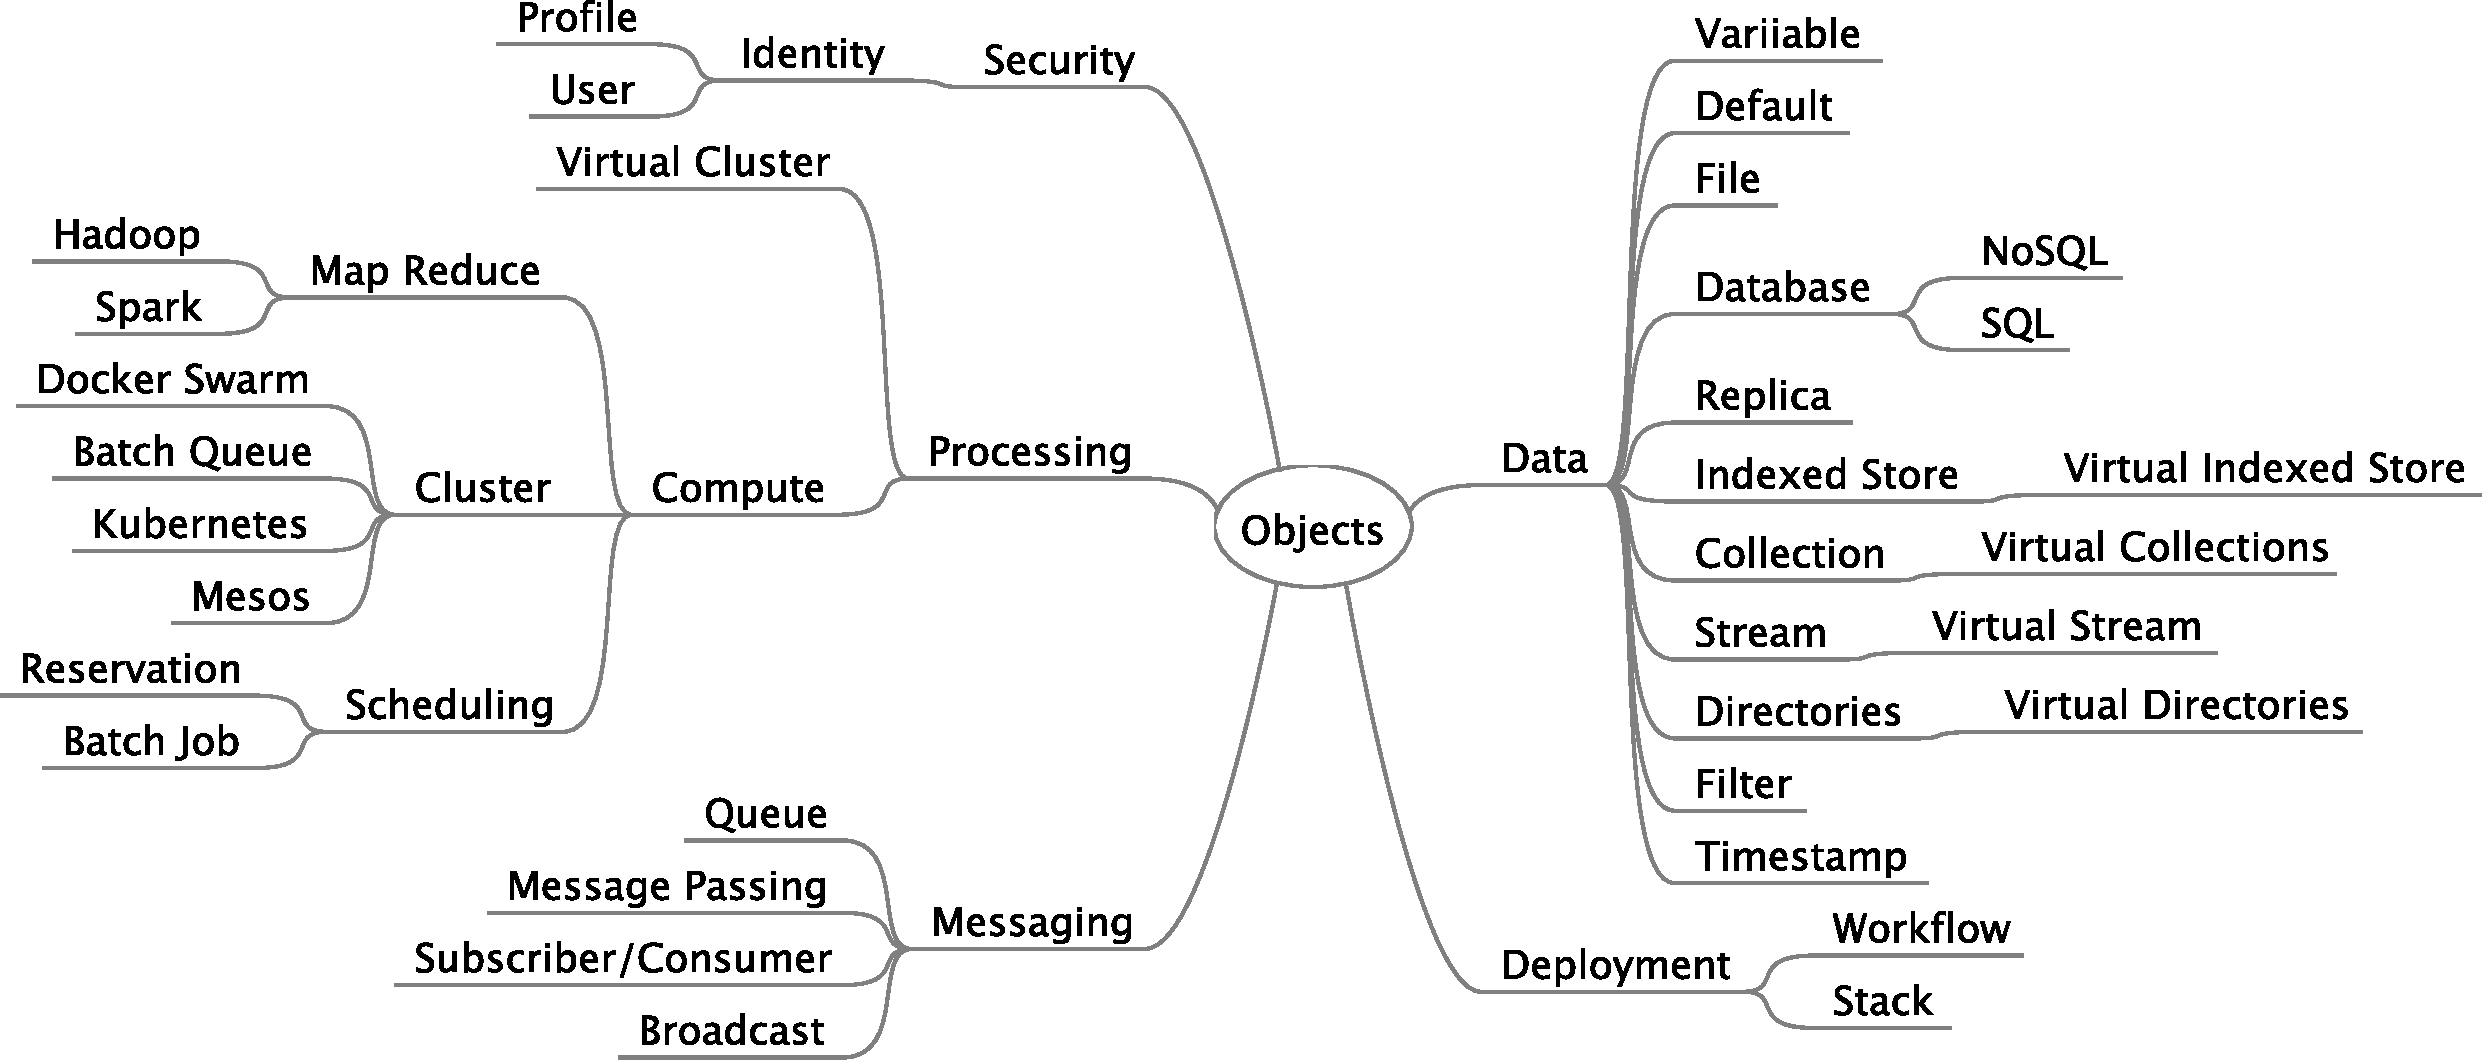
\includegraphics[width=1.1\textwidth]{images/interfaces}
\caption{NIST Big Data Reference Architecture Interfaces}
\label{F:interfaces}
\end{figure*}


\subsection{Identity}

In a multiuser environment, a simple mechanism is used in this document for
associating objects and data to a particular person or group. While 
these efforts do not intend to replace more elaborate solutions such as proposed
by eduPerson \cite{www-eduperson} or others, a very simple way
was chosen to distinguish users. Therefore, the following sections introduce a number of
simple objects including a profile and a user.

\subsubsection{Profile}

A profile defines the identity of an individual. It contains name and
e-mail information. It may have an optional unique user ID (uuid) and/or use a unique
e-mail to distinguish a user. Profiles are used to identify different
users.

\codeFromJson{json}{profile.json}{Profile}{o:profile}

\subsubsection{User}

In contrast to the profile, a user contains additional attributes that
define the role of the user within the multiuser system. The user
associates different roles to individuals. These roles potentially
have gradations of responsibility and privilege.

\codeFromJson{json}{user.json}{Organization}{o:user}

\subsubsection{Organization}

An important concept in many applications is the management of a group
of users in an organization that manages a Big Data application or
infrastructure. User group management can be achieved through three concepts. First, it
can be achieved by using the profile and user resources itself as
they contain the ability to manage multiple users as part of the REST
interface. The second concept is to create a (virtual) organization that
lists all users within the virtual organization. The third concept is to
introduce groups and roles either as part of the user definition or as
part of a simple list similar to the organization.

\codeFromJson{json}{organization.json}{User}{o:organization}

The  profile, user, and organization concepts allow for the clear definition of 
various roles such as
data provider, data consumer, data curator, and others. These concepts also
allow for the creation of services that restrict data access by role, or
organizational affiliation.


\subsubsection{Group/Role}

A group contains a number of users. It is used to manage authorized
services.

\codeFromJson{json}{group.json}{Group}{o:group}

A role is a further refinement of a group. Group members can have specific 
roles. For example, a group of users can be assigned a role that allows 
access to a repository. More specifically, the role would define a user’s 
read and write privileges to the data within the repository.

\codeFromJson{json}{role.json}{Role}{o:role}

%%%%%%%%%%%%%%%%%%%%%%%%%%%%%%%%%%%%%%%%%%%%%%%%%%%%%%%%%%%%%%%%%%%%%%
\subsection{Data}
%%%%%%%%%%%%%%%%%%%%%%%%%%%%%%%%%%%%%%%%%%%%%%%%%%%%%%%%%%%%%%%%%%%%%%

Data for Big Data applications are delivered through data
providers. They can be either local providers contributed by a user or
distributed data providers that refer to data on the internet. At this
time we focus on an elementary set of abstractions related to data
providers that offer us to utilize variables, files, virtual data
directories, data streams, and data filters.

\begin{description}
\item[Variables] are used to hold specific contents that is associated
  in programming language as a variable. A variable has a name, value
  and type.

\item[Defaults] are special type of variables that allow adding of a
  context. Defaults can created for different contexts.

\item[Files] are used to represent information collected within the
  context of classical files in an operating system.

\item[Directories] are locations for storing and organizing multiple
  files on a compute resource.

\item[Virtual Directories] are collection
  of endpoints to files. Files in a virtual directory may be located
  on different resources. For our initial purpose the distinction
  between virtual and non-virtual directories is non-essential and we
  will focus on abstracting all directories to be virtual. This could
  mean that the files are physically hosted on different
  disks. However, it is important to note that virtual data
  directories can hold more than files, they can also contain data
  streams and data filters. 

\item[Streams] are services that offer the consumer a stream of
  data. Streams may allow the initiation of filters to reduce the
  amount of data requested by the consumer.  Stream Filters operate in
  streams or on files converting them to streams.

\item[Batch Filters] operate on streams and on files while working in
  the background and delivering as output Files. In contrast to
  Streams Batch filters process on the data set and return after all
  operations have been applied.

\item[Indexed Stores] are storage systems that store objects and can be
  accessed by an index for each objects. Search and Filter functions
  are integrated to allow identifying objects from it.

\item[Databases] are traditional but also NoSQL databases.

\item[Collections] are agglomeration of any type of data.

\item[Replicas] are duplication of data objects in order to avoid
  overhead due to network or other physical restrictions on a remote
  resource.

\end{description}


\subsubsection{TimeStamp}

Often data needs to be time stamped to indicate when it has been
accessed, created, or modified. All objects defined in this document
will have, in their final version, a time stamp.

\codeFromJson{json}{timestamp.json}{Timestamp}{o:timestamp}

\subsubsection{Variables}

Variables are used to store simple values. Each variable can have a
type, which is also provided as demonstrated in the object below. The
variable value format is defined as string to allow maximal
probability. 

\codeFromJson{json}{var.json}{Var}{o:var}

\subsubsection{Default}

A default is a special variable that has a context associated with
it. This allows one to define values that can be easily retrieved
based on its context. A good example for a default would be the image
name for a cloud where the context is defined by the cloud name.

\codeFromJson{json}{default.json}{Default}{o:default}


\begin{figure}[!h]
\centering
\includegraphics[width=0.5\columnwidth]{images/uml/boot.pdf}
\caption{Booting a VM from defaults}\label{F:uml-boot}
\end{figure}


\subsubsection{File}

A file is a computer resource allowing storage of data that is being
processed. The interface to a file provides the mechanism to
appropriately locate a file in a distributed system. File identification
includes the name, endpoint, checksum, and size. Additional
parameters, such as the last access time, could also be stored. 
The interface only describes the location of the file.

The \textit{file} object has \textit{name}, \textit{endpoint}
(location), \textit{size} in GB, MB, Byte, \textit{checksum} for
integrity check, and last \textit{accessed} timestamp.

\codeFromJson{json}{file.json}{File}{o:file}

\subsubsection{Alias}

A data object could have one alias or even multiple ones. The reason for an
alias is that a file may have a complex name but a user may want to
refer to that file in a name space that is suitable for the user's
application.

\codeFromJson{json}{file_alias.json}{File alias}{o:file-alias}

\subsubsection{Replica}

In many distributed systems, it is of importance that a file can be
replicated among different systems in order to provide faster access.
It is important to provide a mechanism that allows to trace the
pedigree of the file while pointing to its original source. A replica
can be applied to all data types introduced in this document.

\codeFromJson{json}{replica.json}{Replica}{o:replica}


\subsubsection{Virtual Directory}

A collection of files or replicas. A virtual directory can contain an
number of entities including files, streams, and other virtual
directories as part of a collection. The element in the collection can
either be defined by uuid or by name. 

\codeFromJson{json}{virtual_directory.json}{Virtual
  directory}{o:virtual-directory}

\subsubsection{Database}

A \textit{database} could have a name, an \textit{endpoint} (e.g., host, port),
and a protocol used (e.g., SQL, mongo).

\codeFromJson{json}{database.json}{Database}{o:database}

\subsubsection{Stream} 

The stream object describes a data flow, providing information about
the rate and number of items exchanged while issuing requests to the
stream. A stream may return data items in a specific format that is
defined by the stream. 

\codeFromJson{json}{stream.json}{Stream}{o:stream}

Examples for streams could be a stream of random numbers but could
also include more complex formats such as the retrieval of data
records. Services can subscribe and unsubscribe from a stream, while also
applying filters to the subscribed stream.


\subsubsection{Filter} 

Filters can operate on a variety of objects and reduce the
information received based on a search criterion.

\codeFromJson{json}{filter.json}{Filter}{o:filter}


%%%%%%%%%%%%%%%%%%%%%%%%%%%%%%%%%%%%%%%%%%%%%%%%%%%%%%%%%%%%%%%%%%%%%%
\subsection{Virtual Cluster}\label{S:vc}
%%%%%%%%%%%%%%%%%%%%%%%%%%%%%%%%%%%%%%%%%%%%%%%%%%%%%%%%%%%%%%%%%%%%%%

One of the essential features for Big Data is the creation of a Big
Data analysis cluster. A virtual cluster combines resources that
generally are used to serve the Big Data application and can constitute
a variety of data analysis nodes that together build the virtual
cluster. Instead of focusing only on the deployment of a physical
cluster, the creation of a virtual cluster can be instantiated on a
number of different platforms. Such platforms include clouds,
containers, physical hardware, or a mix thereof to support different
aspects of the Big Data application. 

Figure~\ref{F:uml-virtualcluster} illustrates the process for
allocating and provisioning a virtual cluster. The user defines the
desired physical properties of the cluster (e.g., CPU, memory, disk) and
the intended configuration (e.g., software, users). After
requesting the stack to be deployed, cloudmesh allocates the machines
by matching the desired properties with the available
images and booting. The stack definition is then parsed then evaluated
to provision the cluster.


\begin{figure}[!h]
\centering
\includegraphics[width=0.5\columnwidth]{images/uml/virtualcluster.pdf}
\caption{Allocating and provisioning a virtual cluster}\label{F:uml-virtualcluster}
\end{figure}


\subsubsection{Virtual Cluster}

A virtual cluster is an agglomeration of virtual compute nodes that

constitute the cluster. Nodes can be assembled to be baremetal,
VMs, and containers. A virtual cluster contains a number
of virtual compute nodes.  

The virtual cluster object has name, label, endpoint, and provider. The
\textit{endpoint} defines a mechanism to connect to it. The
\textit{provider} defines the nature of the cluster (e.g., it is a
virtual cluster on an OpenStack cloud, or from AWS, or a bare-metal
cluster).

To manage the cluster it can have a frontend node that is used to
manage other nodes. Authorized keys within the definition of the
cluster allow administrative functions, while authorized keys on a
compute node allow login and use functionality of the virtual nodes.

\codeFromJson{json}{virtual_cluster.json}{Virtual
  cluster}{o:virtual-cluster}

\codeFromJson{json}{virtual_cluster_provider.type}{Virtual
  cluster provider}{o:virtual-cluster-provider}

% \codeFromJson{json}{cluster.json}{Cluster}{o:cluster}

\subsubsection{Compute Node}

Compute nodes are used to conduct compute and data functions. They are
of a specific {\it kind}. For example,compute nodes could be a virtual machine
(VM), bare metal, or part of a predefined virtual cluster
framework. 

Compute nodes are a representation of a computer system (physical or
virtual). A very basic set of information about the compute node is maintained in this document. 
It is expected that, through the endpoint, the VM can be
introspected and more detailed information can be retrieved. A compute
node has name, label, a flavor, network interface cards (NICs) and other relevant information.


\codeFromJson{json}{virtual_machine.json}{Compute node of a virtual cluster}{o:virtual-machine}

\subsubsection{Flavor}

The flavor specifies elementary information about the compute node,
such as memory and number of cores, as well as other attributes that can
be added. Flavors are essential to size a virtual cluster appropriately.

\codeFromJson{json}{flavor.json}{Flavor}{o:flavor}


%
% BEGIN OLD
%
% \codeFromJson{json}{virtual_compute_node.json}{Compute node}{o:virtual-compute-node}
% \codeFromJson{json}{compute_resource.json}{Compute resource}{o:compute-resource}
% \codeFromJson{json}{computer.json}{Computer}{o:computer}
%
% END OLD
%

\subsubsection{Network Interface Card}

To interact between the nodes, a network interface is needed. Such a
network interface, specified on a virtual machine with a NIC
object, is showcased in Object~\ref{o:nic}. 

\codeFromJson{json}{nic.json}{Network interface card}{o:nic}

\subsubsection{Key}

Many services and frameworks use Secure Shell (SSH) keys to authenticate. To allow
the convenient storage of the public key, the sshkey object can be
used (see Object \ref{o:key}).

\codeFromJson{json}{sshkey.json}{Key}{o:key}

\subsubsection{Security Groups}

To allow secure communication between the nodes, security groups are
introduced. They define the typical security groups that will be
deployed once a compute node is specified. The security group object
is depicted in Object \ref{o:secgroup}.

\codeFromJson{json}{security_group.json}{Security Groups}{o:secgroup}



% BEGIN OLD
%
% THIS IS ACTUALLY NOT A NEW OBJEC BUT AN OLD OBJECT
%
%\subsubsection{New Cluster}
%\codeFromJson{json}{cluster_new.json}{Cluster}{o:cluster-new}
%





% \subsubsection{Compute Node}

% A node is composed of multiple components:

% \begin{enumerate}
% \item Metadata such as the \verb|name| or \verb|owner|.
% \item Physical properties such as \verb|cores| or \verb|memory|.
% \item Configuration guidance such as \verb|create_external_ip|,
%   \verb|security_groups|, or \verb|users|.
% \end{enumerate}

% The metadata is associated with the node on the provider end (if
% supported) as well as in the database. Certain parts of the metadata
% (such as \verb|owner|) can be used to implement access
% control. Physical properties are relevant for the initial allocation
% of the node. Other configuration parameters control and further
% provisioning.

% In the above, after allocation, the node is configured with a user
% called \verb|hello| who is part of the \verb|wheel| group whose
% account can be accessed with several SSH identities whose public keys
% are provided (in \verb|authorized_keys|).

% Additionally, three ssh keys are generated on the node for the
% \verb|hello| user. The first uses the \verb|ed25519| cryptographic
% method with a password read in from a GPG-encrypted file on the
% Command and Control node. The second is a 4098-bit RSA key also
% password-protected from the GPG-encrypted file. The third key is
% copied to the remote node from an encrypted file on the Command and
% Control node.

% This definition also provides a security group to control access to
% the node from the wide-area-network. In this case all ingress and
% egress TCP and UDP traffic is allowed provided they are to ports 22
% (SSH), 443 (SSL), and 80 and 8080 (web).


% \codeFromJson{json}{node.json}{Node}{o:node}

% \codeFromJson{json}{node-new.json}{Node}{o:node}

% END OLD


%%%%%%%%%%%%%%%%%%%%%%%%%%%%%%%%%%%%%%%%%%%%%%%%%%%%%%%%%%%%%%%%%%%%%%
\subsection{Infrastructure as a Service}
%%%%%%%%%%%%%%%%%%%%%%%%%%%%%%%%%%%%%%%%%%%%%%%%%%%%%%%%%%%%%%%%%%%%%%

Although Section \ref{S:vc} defines a general virtual
cluster useful for Big Data, sometimes the need exists to
specifically utilize Infrastructure as a Service (IaaS) frameworks, such as
Openstack, Azure, and others. To do so, it is beneficial to
be able to define virtual clusters using these frameworks. Hence, 
this subsection defines interfaces related to 
IaaS frameworks. This includes specific objects useful for
OpenStack, Azure, and AWS, as well as others. The definition of the
objects used between the clouds to manage them, are different and not
standardized. In this case the objects support functions such as

starting, stoping, suspending resuming, migration, network
configuration, assigning of resources, assigning of operating systems
for and others for the VMs.

Inspecting other examples, such as {\it LibCloud}, shows the definition of
generalized objects are discovered, which are augmented with extra fields to
specifically integrate with the various frameworks. When working with
cloudmesh, it is sufficient to be able to specify a
cloud based on a cloud specific action. Actions include boot,
terminate, suspend, resume, assign network intrusion prevention system, and add users.

To support such actions, objects can be selected based on the
IaaS type in use when invoked. The following subsections list these objects as used in
LibCloud, OpenStack, and Azure. 

% ----------------------------------------------------------------------
\subsubsection{LibCloud}
% ----------------------------------------------------------------------

Libcloud is a Python library for interacting with different cloud
service providers. It uses a unified API that exposes similar access
to a variety of clouds. Internally, it uses objects that can
interface with different IaaS frameworks. However, as these frameworks
are different from each other, specific adaptations are done for
each IaaS, mostly reflected in the LibCloud Node (see Section
\ref{S:libcloudnode})

\paragraph{Challenges}

For time considerations, LibCloud was used for some time practically in various versions of
cloudmesh. However, it became apparent that at times the representation and
functionality provided by LibCloud, for reference implementations, did
not support some advanced aspects provided by the native cloud
objects. Depending on the application, libraries for interfacing with different frameworks, 
direct utilization of the native
objects, and interfaces provided by a particular IaaS framework could all be viable options. 
Additional interfaces have been introduced in
Sections \ref{S:openstack} and \ref{S:azure}. 
Additional sections addressing other IaaS frameworks may be integrated in the future.

\paragraph{LibCloud Flavor}

The object referring to flavors is listed in Object \ref{o:libcloud-flavor}.

\codeFromJson{json}{libcloud_flavor.json}{Libcloud flavor}{o:libcloud-flavor}

\paragraph{LibCloud Image}

The object referring to images is listed in Object
\ref{o:libcloud-images}.

\codeFromJson{json}{libcloud_image.json}{Libcloud image}{o:libcloud-image}


\paragraph{LibCloud VM}


The object referring to virtual machines is listed in 


\codeFromJson{json}{libcloud_vm.json}{LibCloud VM}{o:libcloud-vm}

\paragraph{LibCloud Node}\label{S:libcloudnode}


Virtual machines for the various clouds have additional attributes
that are summarized in Object \ref{o:libcloud-vm}. These attributes 
will be integrated into the VM object in the future.

\codeFromJson{json}{libcloudNode.json}{LibCloud Node}{o:libcloud-node}


% ----------------------------------------------------------------------
\subsubsection{OpenStack}\label{S:openstack}
% ----------------------------------------------------------------------

Objects related to OpenStack VMs are summarized in this
section.

\paragraph{OpenStack Flavor}

The object referring to flavors is listed in Object
\ref{o:libcloud-flavor}.

\codeFromJson{json}{openstack_flavor.json}{Openstack flavor}{o:openstack-flavor}

\paragraph{OpenStack Image}

The object referring to images is listed in Object
\ref{o:openstack-image}.

\codeFromJson{json}{openstack_image.json}{Openstack
  image}{o:openstack-image}

\paragraph{OpenStack VM}

The object referring to VMs is listed in Object \ref{o:openstack-vm}.


\codeFromJson{json}{openstack_vm.json}{Openstack
  vm}{o:openstack-vm}

% ----------------------------------------------------------------------
\subsubsection{Azure}\label{S:azure}
% ----------------------------------------------------------------------

Objects related to Azure virtual machines are summarized in this
section.

\paragraph{Azure Size}

The object referring to the image size machines is listed in Object \ref{o:azure-size}.

\codeFromJson{json}{azure-size.json}{Azure-size}{o:azure-size}


\paragraph{Azure Image}

The object referring to the images machines is listed in Object
\ref{o:azure-image}.

\codeFromJson{json}{azure-image.json}{Azure-image}{o:azure-image}

\paragraph{Azure VM}

The object referring to the virtual machines is listed in Object
\ref{o:azure-vm}.
 
\codeFromJson{json}{azure-vm.json}{Azure-vm}{o:azure-vm}


%%%%%%%%%%%%%%%%%%%%%%%%%%%%%%%%%%%%%%%%%%%%%%%%%%%%%%%%%%%%%%%%%%%%%%
\subsection{Compute Services}
%%%%%%%%%%%%%%%%%%%%%%%%%%%%%%%%%%%%%%%%%%%%%%%%%%%%%%%%%%%%%%%%%%%%%%

\subsubsection{Batch Queue}

Computing jobs that can run without end user interaction, or are
scheduled based on resource permission are called batch jobs. It is
used to minimize human interaction and allows the submission and
scheduling of many jobs in parallel while attempting to utilize the
resources through a resource scheduler more efficiently or simply in
sequential order. Batch processing is not to be underestimated even in
todays shifting IoT environment towards clouds and containers. This is
based on the fact that for some application resources managed by batch
queues are highly optimized and in many cases provide significant
performance advantages. Disadvantages are the limited and preinstalled
software stacks that in some cases do not allow to run the latests
applications.

\codeFromJson{json}{batchjob.json}{Batchjob}{o:batchjob}

%%%%%%%%%%%%%%%%%%%%%%%%%%%%%%%%%%%%%%%%%%%%%%%%%%%%%%%%%%%%%%%%%%%%%%
\subsubsection{Reservation}
%%%%%%%%%%%%%%%%%%%%%%%%%%%%%%%%%%%%%%%%%%%%%%%%%%%%%%%%%%%%%%%%%%%%%%

Some services may consume a considerable amount of resources, necessitating
the reservation of resources. For this purpose, a reservation object (Object \ref{o:reservation}) has been introduced.

\codeFromJson{json}{reservation.json}{Reservation}{o:reservation}


\begin{comment}
\subsubsection{Mesos}

\TODO{Refine}

\codeFromJson{json}{mesos.json}{Mesos}{o:mesos}
\end{comment}

%%%%%%%%%%%%%%%%%%%%%%%%%%%%%%%%%%%%%%%%%%%%%%%%%%%%%%%%%%%%%%%%%%%%%%
\subsection{Containers}
%%%%%%%%%%%%%%%%%%%%%%%%%%%%%%%%%%%%%%%%%%%%%%%%%%%%%%%%%%%%%%%%%%%%%%

The following defines the {\em container} object. 

\codeFromJson{json}{container.json}{Container}{o:container}

\begin{comment}
\subsubsection{Kubernetes}

\TODO{REFINE}

\codeFromJson{json}{kubernetes.json}{Kubernetes}{o:kubernetes}
\end{comment}

%%%%%%%%%%%%%%%%%%%%%%%%%%%%%%%%%%%%%%%%%%%%%%%%%%%%%%%%%%%%%%%%%%%%%%
\subsection{Deployment}
%%%%%%%%%%%%%%%%%%%%%%%%%%%%%%%%%%%%%%%%%%%%%%%%%%%%%%%%%%%%%%%%%%%%%%

A \textit{deployment} consists of the resource \- \textit{cluster},
the location \- \textit{provider} (e.g., OpenStack), and
software \textit{stack} to be deployed (e.g., Hadoop, Spark).

\codeFromJson{json}{deployment.json}{Deployment}{o:deployment}

%%%%%%%%%%%%%%%%%%%%%%%%%%%%%%%%%%%%%%%%%%%%%%%%%%%%%%%%%%%%%%%%%%%%%%
\subsection{Mapreduce}
%%%%%%%%%%%%%%%%%%%%%%%%%%%%%%%%%%%%%%%%%%%%%%%%%%%%%%%%%%%%%%%%%%%%%%

The \textit{mapreduce} deployment has as inputs parameters defining
the applied function and the input data.  Both function and data
objects define a ``source'' parameter, which specify the location it
is retrieved from. For instance, the ``file://'' URI indicates sending
a directory structure from the local file system where the ``ftp://''
indicates that the data should be fetched from a FTP resource. It is
the framework's responsibility to materialize and instantiation of the
desired environment along with the function and data.

\codeFromJson{json}{mapreduce.json}{Mapreduce}{o:mapreduce}

Additional parameters include the ``fault\_tolerant'' and ``backend''
parameters.  The former flag indicates if the \textit{mapreduce}
deployment should operate in a fault tolerant mode. For instance, in
the case of Hadoop, this may mean configuring automatic failover of
name nodes using Zookeeper.  The ``backend'' parameter accepts an
object describing the system providing the \textit{mapreduce}
workflow.  This may be a native deployment of Hadoop, or a special
instantiation using other frameworks such as Mesos.

A function prototype is defined in Listing~\ref{o:mr.f.prototype}.
Key properties are that functions describe their input parameters and
generated results. For the former, the ``buildInputs'' and
``systemBuildInputs'' respectively describe the objects which should
be evaluated and system packages which should be present before this
function can be installed. The ``eval'' attribute describes how to
apply this function to its input data. Parameters affecting the
evaluation of the function may be passed in as the ``args'' attribute.
The results of the function application can be accessed via the
``outputs'' object, which is a mapping from arbitrary keys
(e.g. ``data'', ``processed'', ``model'') to an object representing
the result.

\codeFromJson{json}{mapreduce_function_prototype.json}{Mapreduce function}{o:mr.f.prototype}


Some example functions include the ``NoOp'' function shown in
Listing~\ref{o:mr.f.noop}.  In the case of undefined arguments,
the parameters default to an identity element. In the case of mappings
this is the empty mapping while for lists this is the empty list.

\codeFromJson{json}{mapreduce_function_noop.json}{Mapreduce noop}{o:mr.f.noop}


\subsubsection{Hadoop}

A \textit{hadoop} definition defines which \textit{deployer} to be used,
the \textit{parameters} of the deployment, and the system packages as
\textit{requires}. For each requirement, it could have attributes such
as the library origin, version, and others (see Object \ref{o:hadoop})

\codeFromJson{json}{hadoop.json}{Hadoop}{o:hadoop}


%%%%%%%%%%%%%%%%%%%%%%%%%%%%%%%%%%%%%%%%%%%%%%%%%%%%%%%%%%%%%%%%%%%%%%
\subsection{Microservice}
%%%%%%%%%%%%%%%%%%%%%%%%%%%%%%%%%%%%%%%%%%%%%%%%%%%%%%%%%%%%%%%%%%%%%%

As part of microservices, a function with parameters that can be invoked
has been defined. To describe such services, the Object \ref {o:microservice}
was created. Defining multiple services facilitates the finding of the
microservices and the use as part of a microservice based implementation.
 
\codeFromJson{json}{microservice.json}{Microservice}{o:microservice}



 
%%%%%%%%%%%%%%%%%%%%%%%%%%%%%%%%%%%%%%%%%%%%%%%%%%%%%%%%%%%%%%%%%%%%%%
\subsubsection{Accounting}
%%%%%%%%%%%%%%%%%%%%%%%%%%%%%%%%%%%%%%%%%%%%%%%%%%%%%%%%%%%%%%%%%%%%%%


As in big data applications and systems considerable amount of
resources are used an accounting system must be present either on the
server side or on the application and user side to allow checking of
balances. Due to the potential heterogeneous nature of the services
used existing accounting frameworks may not be present to dela with
this issue. E.g. we see potentially the use of multiple accounting
systems with different scales of accuracy information feedback
rates. For example, if the existing accounting system informs the user
only hours after she has started a job this could pose a significant
risk because charging is started immediately. While making access to
big data infrastructure and services more simple, the user or
application may underestimate the overall cost projected by the
implementation of the big data reference architecture.

\codeFromJson{json}{accounting.json}{Accounting}{o:accounting}

\codeFromJson{json}{account.json}{Account}{o:account}

\paragraph{Usecase: Accounting Service}

Figure \ref{F:create resource} depicts a possible accounting service
that allows an administrator to register a variety of resources to an
account for a user. The services that are than invoked by the user can
than consume the resource and are charged accordingly.

\begin{figure}[!h]
\includegraphics[width=0.8\columnwidth]{images/dot/account.pdf}
\caption{Create Resource}\label{F:createresource}
\end{figure}

\begin{figure}[!h]
\centering
\includegraphics[height=0.8\textheight]{images/uml/account.pdf}
\caption{Accounting}\label{F:uml-accounting}
\end{figure}



\begin{comment}

%%%%%%%%%%%%%%%%%%%%%%%%%%%%%%%%%%%%%%%%%%%%%%%%%%%%%%%%%%%%%%%%%%%%%%
\subsection{Network}
%%%%%%%%%%%%%%%%%%%%%%%%%%%%%%%%%%%%%%%%%%%%%%%%%%%%%%%%%%%%%%%%%%%%%%

\TODO{We are looking for volunteers to contribute to the network section.}

\end{comment}

%\bibliography{references}

\section{Status Codes and Error Responses}

In case of an error or a successful response, the response header
contains a HTTP code (see
\url{https://tools.ietf.org/html/rfc7231}). The response body usually
contains

\begin{itemize}
\item the HTTP response code
\item an accompanying message for the HTTP response code
\item a field or object where the error occurred 
\end{itemize}

\begin{table}[!h]
\caption{HTTP response codes}
\begin{tabular}{p{1cm}p{15cm}}
HTTP & response Description code \\
\hline
200 & {\it OK} success code, for GET or HEAD request. \\
201 & {\it Created} success code, for POST request. \\
204 & {\it No Content} success code, for DELETE request. \\
300 & The value returned when an external ID exists in more than one
      record. \\
304 & The request content has not changed since a specified date and
      time. \\
400 & The request could not be understood. \\
401 & The session ID or OAuth token used has expired or is invalid. \\
403 & The request has been refused. \\
404 & The requested resource could not be found. \\
405 & The method specified in the Request-Line is not allowed for the
      resource specified in the URI. \\
415 & The entity in the request is in a format that is not supported by
      the specified method. \\
\end{tabular}
\end{table}

% \url{http://www.restapitutorial.com/httpstatuscodes.html}
% \url{https://en.wikipedia.org/wiki/List_of_HTTP_status_codes}
% \url{http://www.ietf.org/assignments/http-status-codes/http-status-codes.xml}



\clearpage
\newpage

\section{Acronyms and Terms}

The following acronyms and terms are used in the paper

\begin{description}[leftmargin=8em,style=nextline]
\item[ACID] 	       Atomicity, Consistency, Isolation, Durability
\item[API] 	       Application Programming Interface
\item[ASCII] 	       American Standard Code for Information Interchange 
\item[BASE] 	       Basically Available, Soft state, Eventual consistency

\item[Container] see
  \url{http://csrc.nist.gov/publications/drafts/800-180/sp800-180_draft.pdf}

\item[Cloud Computing] the practice of using a network of remote
  servers hosted on the Internet to store, manage, and process data,
  rather than a local server or a personal computer. See \url{http://nvlpubs.nist.gov/nistpubs/Legacy/SP/nistspecialpublication800-145.pdf}

\item[DevOps] 	       A clipped compound of {\em software DEVelopment} and
                       {\em information technology OPerationS}
\item[Deployment]      The action of installing software on resources.

\item[HTTP] 	       HyperText Transfer Protocol HTTPS HTTP Secure

\item[Hybrid Cloud] See
  \url{http://nvlpubs.nist.gov/nistpubs/Legacy/SP/nistspecialpublication800-145.pdf}

\item[IaaS] 	       Infrastructure as a Service SaaS Software as a Service

\item[ITL] 	       Information Technology Laboratory

\item[Microservice Architecture] Is an approach to build applications
  based on many smaller modular services. Each module supports a
  specific goal and uses a simple, well-defined interface to
  communicate with other sets of services.

\item[NBD-PWG]	       NIST Big Data Public Working Group

\item[NBDRA] 	       NIST Big Data Reference Architecture 

\item[NBDRAI] 	       NIST Big Data Reference Architecture Interface

\item[NIST] 	       National Institute of Standards

\item[OS] 	       Operating System

\item[REST] 	       REpresentational State Transfer

\item[Replica] A duplicate of a file on another resource in
  order to avoid costly transfer costs in case of frequent access.

\item[Serverless Computing] Serverless computing specifies the
  paragdigm of function as a service (FaaS). It is a cloud computing
  code execution model in which a cloud provider manages the function
  deployment and utilization while clients can utilize them. The
  charge model is based on execution of the function rather than the
  cost to manage and host the VM or container.

\item[Software Stack] A set of programs and services that are
  installed on a resource in order to support applications.

\item[Virtual Filesysyem] An abstraction layer on top of a 
  a distributed physical file system to allow easy access to the files
  by the user or application.

\item[Virtual Machine] A VM is a software computer that,
  like a physical computer, runs an operating system and applications.
  The VM is comprised of a set of specification and
  configuration files and is backed by the physical resources of a
  host.

\item[Virtual Cluster] A virtual cluster is a software cluster that
  integrate either VMs, containers or physical resources into an
  agglomeration of compute resources. A virtual cluster allows user
  sto authenticate and authorize to the virtual compute nodes tu
  utilize them for calculations. Optional high level services that can
  be deployed on a virtual cluster may simplify
  interaction with the virtual cluster or provide higher level
  services. 

\item[Workflow] the sequence of processes or tasks

\item[WWW] World Wide Web

\end{description}
 

\newpage

%\bibliographystyle{styles/IEEEtran}  
\bibliographystyle{styles/plainurl}  
\bibliography{references}

\newpage

\appendix

%%%%%%%%%%%%%%%%%%%%%%%%%%%%%%%%%%%%%%%%%%%%%%%%%%%%%%%%%%%%%%%%%%%%%%
\section{Appendix}
%%%%%%%%%%%%%%%%%%%%%%%%%%%%%%%%%%%%%%%%%%%%%%%%%%%%%%%%%%%%%%%%%%%%%%

\subsection{Schema}\label{s:schema}

Listing \ref{l:schema} showcases the schema generated from the objects
defined in this document.

\codeFromJson{python}{../settings.settings.py}{Schema}{l:schema}

\section{Cloudmesh Rest}\label{s:cloudmesh-rest}

Cloudmesh Rest is a reference implementation for the NBDRA. It
allows for automatic definition of a REST service based on the objects
specified by the NBDRA. In collaboration with other cloudmesh
components it allows easy interaction with hybrid clouds and the
creation of user managed Big Data services. 

\subsection{Prerequisites}\label{prerequistis}

The prerequisiits for cloudmesh Rest are Python 2.7.13 or 3.6.1.
It can easily be installed on a variety of systems (at this time
only ubuntu greater 16.04 and OSX Sierra have been tested). However, it would
naturally be possible to also port it to Windows. At the time of publication, the installation
instructions in this document are not complete. The reader is
referred to the cloudmesh manuals, which are under development. The goal
will be to make the installation (after the system is set up for
developing Python) as simple as the following:

\begin{verbatim}
    pip install cloudmesh.rest
\end{verbatim}


\subsection{REST Service}\label{cm-rest}

With the cloudmesh REST framework, it is easy to create REST services
while defining the resources via example JSON objects. This is achieved
while leveraging the Python eve \cite{www-eve} and a modified version of Python
evengine \cite{www-cloudmesh-eveengine}. 

A valid JSON resource specification looks like this:

\begin{verbatim}
{
  "profile": {
    "description": "The Profile of a user",
    "email": "laszewski@gmail.com",
    "firstname": "Gregor",
    "lastname": "von Laszewski",
    "username": "gregor"
  }
}
\end{verbatim}

In this example, an object called profile is defined, which contains a number of
attributes and values. The type of the values is automatically
determined. All JSON specifications are contained in a directory and
can easily be converted into a valid schema for the eve REST service
by executing the following commands:

\begin{verbatim}
cms schema cat . all.json
cms schema convert all.json
\end{verbatim}

This will create the configuration \verb|all.settings.py| that can
be used to start an eve service.

Once the schema has been defined, cloudmesh specifies defaults for managing
a sample database that is coupled with the REST service. 
MongoDB was used which could be placed on a sharded mongo service. 

\subsection{Limitations}

The current implementation is a demonstration and showcases that it is
easy to generate a fully functioning REST service based on the
specifications provided in this document. However, it is expected that
scalability, distribution of services, and other advanced options
need to be addrassed based on application requirements.



\section{Contributing}

We invite you to contribute to this paper and its discussion to
improve it. Improvements can be done with pull requests. We suggest
you do {\em small} individual changes to a single subsection and
object rather than large changes as this allows us to integrate the
changes individually and comment on your contribution via github. Once
contributed we will appropriately acknowledge you either as
contributor or author. Please discuss with us how we best acknowledge
you.


\subsection{Conversion to Word}

We found that it is most convenient to manage the draft document on
github. Currently the document is located at:

\begin{itemize}
\item \url{https://github.com/cloudmesh/cloudmesh.rest/tree/master/docs}
\end{itemize}

Managing the document in github has provided us with the advantage that a
reference implementation can be automatically derived from the
specified objects. Also it is easy to contribute as all text is
written in ASCII while using \LaTeX syntax to allow for formating in
PDF. 

Contributions can be mades as follows:

\begin{description}
\item[Contributions with git pull requests]: You can fork the
  repository, make modifications and create a pull request that we
  than review and integrate
\item[Contribution with direct access]: Cloudmesh.rest developers have
  direct access to the repository. If you are a frequent contributor
  to the document and are familiar with github we can grant you
  access. However, we do prefer pull requests as this minimizes our
  administrative overhead to avoid issues with git
\item[Contributing ASCII sections with git issues]: You can identify
  the version of the document, specify the section and line numbers
  you want to modify and include the new text. We will integrate and
  address these issues ASAP. Issues can be submitted at 
  \url{https://github.com/cloudmesh/cloudmesh.rest/issues}
\end{description}


\subsection{Object Specification}

All objects are located in 

\begin{verbatim}
cloudmesh.rest/cloudmesh/specification/examples
\end{verbatim}

And can be modified there

\subsection{Creation of the PDF document}

We assume that you have LaTeX installed. Latex can be trivially
installed on Windows, OSX, and Linux. Please refer to the instalation
instructions for your OS. If you have Windows and have not make installed, you can
obtain it from \url{http://gnuwin32.sourceforge.net/packages/make.htm}
Please google for it and find the version most suitable for you.

Firts you have to obtain the document from github.com. Currently, you
can do this with 

\begin{verbatim}
   git clone https://github.com/cloudmesh/cloudmesh.rest
\end{verbatim}

To compile the document please use 

\begin{verbatim}
   cd docs
   make
\end{verbatim}

This will generate the PDF file 

\begin{verbatim}
   NIST.SP.1500-8-draft.pdf
\end{verbatim}

On OSX we have also integrated a quick view whit 

\begin{verbatim}
   make view
\end{verbatim}

The PDF document can be transfered to doc and docx, with the following
online tool:

* \url{http://pdf2docx.com/}

We noticed that some tabs in the object definitions may get lost, but
they can be integrated easily. If yo notice any other formatting
issues, please file an issue.

We assume that those writeing the document in word use a simple style
theme using regular styles. Once the NIST editors have provided a
suitable style them we will upload it to the repository so it can be
applied easily.

\subsection{Code Generation}

This section is intended for experts and guidance on using it can be
obtained by contacting Gregor von Laszewski. It is assumed that you
have installed all the tools. To create the document you can simply do

\begin{Verbatim}
git clone https://github.com/cloudmesh/cloudmesh.rest
python setup.py install; pip install .
cd cloudmesh.rest
cd docs
make schema
make
\end{Verbatim}

This will produce in that directory a file called object.pdf
containing this document. 

\end{document}
%
